% Author: Till Tantau
% Source: The PGF/TikZ manual

\documentclass{article}

\usepackage{pgf}
\usepackage{tikz}
\usetikzlibrary{arrows,automata}
\usepackage[latin1]{inputenc}
\usepackage{verbatim}

\begin{document}



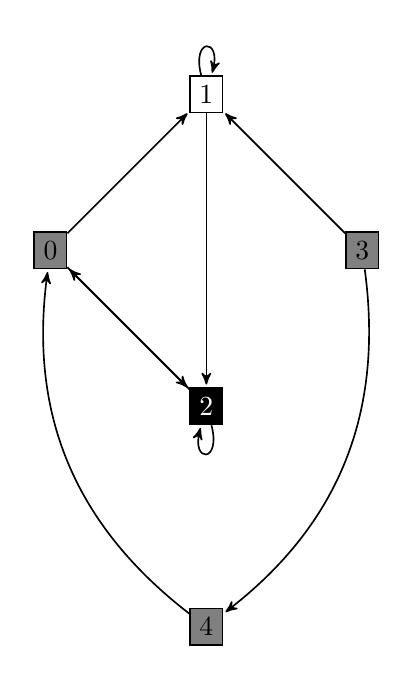
\begin{tikzpicture}[->,>=stealth',shorten >=1pt,auto,node distance=2.8cm,
                    semithick]
  \tikzstyle{wstate}=[fill=white,text=black,draw=black]
  \tikzstyle{gstate}=[fill=gray,text=black,draw=black]
  \tikzstyle{bstate}=[fill=black,text=white,draw=black]
  
  \node[gstate] 		(0)                    {$0$};
  \node[wstate]         (1) [above right of=0] {$1$};
  \node[bstate]         (2) [below right of=0] {$2$};
  \node[gstate]         (3) [below right of=1] {$3$};
  \node[gstate]         (4) [below of=2]       {$4$};

  \path (0) edge              node {} (1)
            edge              node {} (2)
        (1) edge [loop above] node {} (1)
            edge              node {} (2)
        (3) edge              node {} (1)
            edge [bend left]  node {} (4)
        (2) edge [loop below] node {} (2)
            edge              node {} (0)
        (4) edge [bend left]  node {} (0);
\end{tikzpicture}

\end{document}